\documentclass{standalone}
\usepackage{tikz}
\usepackage{pgfplots}
\pgfplotsset{compat=newest}
\usepackage{amsmath}
\usepackage[american]{circuitikz}
\usepackage{cmbright}

\ctikzset{bipoles/resistor/height=0.2, bipoles/resistor/width=0.6}

\definecolor{myred}{RGB}{170,0,0}
\definecolor{myblue}{RGB}{0,0,220}
\definecolor{mygreen}{RGB}{0,150,0}
\definecolor{myorange}{RGB}{255,127,0}
\definecolor{mybrown}{RGB}{150,75,0}

\begin{document}
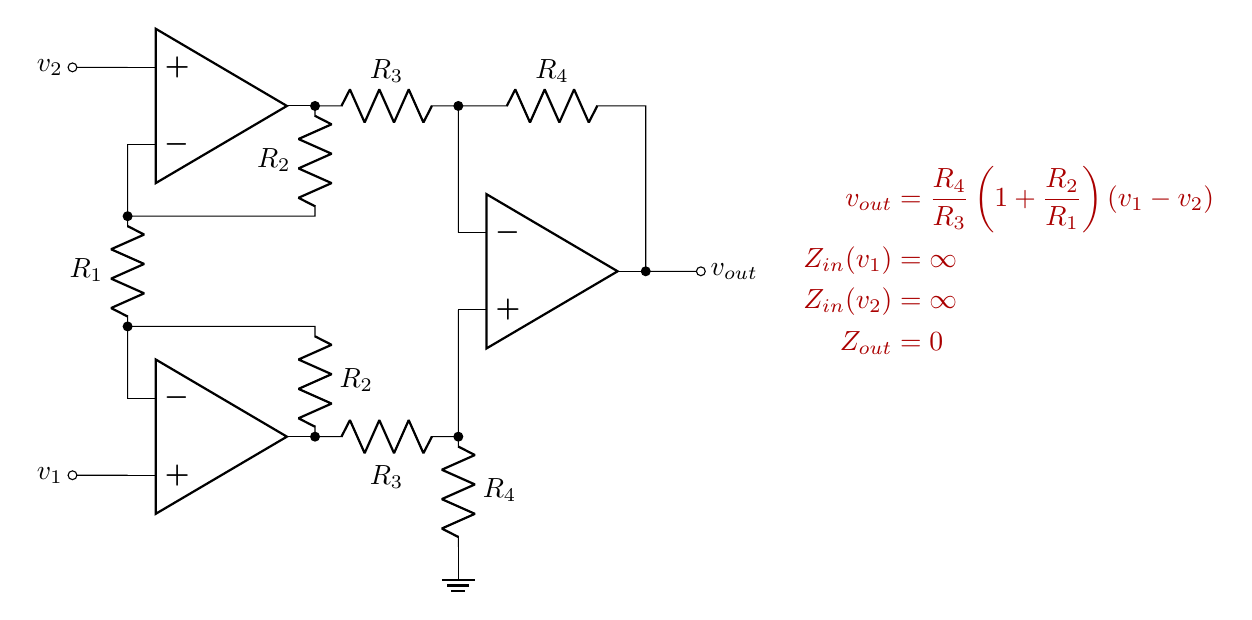
\begin{tikzpicture}
    \begin{scope}[scale=0.7]
        \draw (0, 0) node[op amp, yscale=-1] (OpAmp1) {};
        \draw (0, -6) node[op amp] (OpAmp2) {};
        \draw (6, -3) node[op amp] (OpAmp3) {};
        \path let \p1 = (OpAmp1.+) in
            \pgfextra{
                \xdef\xin{\x1}
                \xdef\yin{\y1}
            };
        \path let \p1 = (OpAmp1.out) in
            \pgfextra{
                \xdef\xout{\x1}
                \xdef\yout{\y1}
            };
        \path let \p1 = (OpAmp3.+) in
            \pgfextra{
                \xdef\ain{\x1}
                \xdef\bin{\y1}
            };
        \path let \p1 = (OpAmp3.-) in
            \pgfextra{
                \xdef\cin{\x1}
                \xdef\din{\y1}
            };
        \path let \p1 = (OpAmp3.out) in
            \pgfextra{
                \xdef\eout{\x1}
                \xdef\fout{\y1}
            };
        \draw (OpAmp1.-)
            to[R, l_={$R_1$}] (OpAmp2.-);
        \draw (OpAmp1.out)
            to[R, l_={$R_2$}, *-] ++(0, -2)
            to[short, -*] ++(\xin - \xout, 0);
        \draw (OpAmp2.out)
            to[R, l_={$R_2$}, *-] ++(0, +2)
            to[short, -*] ++(\xin - \xout, 0);
        \draw (OpAmp1.out)
            to[R, l={$R_3$}, -*] ++(\ain - \xout, 0)
            to[R, l={$R_4$}] ++(\eout - \ain, 0)
            to[short, -*] (OpAmp3.out)
            to[short, -o] ++(1.0, 0)
            node[anchor=west] {$v_{out}$};
        \draw (OpAmp3.-)
            to[short] ++(0, \yout - \din);
        \draw (OpAmp2.out)
            to[R, l_={$R_3$}, -*] ++(\ain - \xout, 0)
            to[R, l={$R_4$}] ++(0, -2)
            node[ground] {};
        \draw ($(OpAmp2.out) + (\ain - \xout, 0)$)
            to[short] (OpAmp3.+);
        \draw (OpAmp1.+)
            to[short, -o] ++(-1.0, 0)
            node[anchor=east] {$v_{2}$};
        \draw (OpAmp2.+)
            to[short, -o] ++(-1.0, 0)
            node[anchor=east] {$v_{1}$};
    \end{scope}
    \begin{scope}[xshift=10.0cm, yshift=-2cm, scale=0.7]
        % Title
        \node[anchor=center, color=myred] at (0, 0) {
            $\begin{aligned}
                v_{out} &= \frac{R_4}{R_3} \left(1 + \frac{R_2}{R_1}\right) \left(v_{1} - v_{2}\right) \\
                Z_{in}(v_1) &= \infty \\
                Z_{in}(v_2) &= \infty \\
                Z_{out} &= 0
            \end{aligned}$
        }; 
    \end{scope}
\end{tikzpicture}
\end{document}